\documentclass{standalone}
\usepackage{tikz,color}
\usepackage[EULERGREEK]{sansmath}
\begin{document}
\sansmath
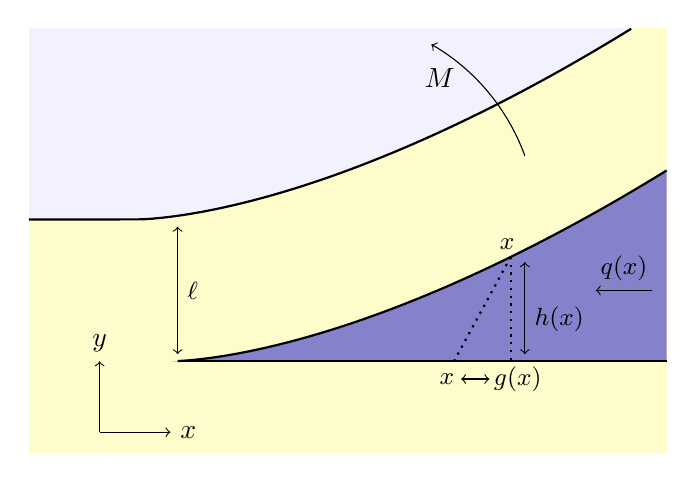
\begin{tikzpicture}[scale=0.9]

\path [fill=blue ,opacity=0.6]
plot [domain=1:70, samples=50, thick ] ( {0.1*\x}, {0.003*pow(\x,1.6)})
|- (0,0);

\path[fill=yellow, opacity=0.2] (-2,-1.3) rectangle (7,4.7);

\path [fill=white]
plot [domain=1:70, samples=50, thick ] ( {0.1*\x-0.5}, {2+0.003*pow(\x,1.6)})
|- (-0.4,4.7);

\path[fill=white, opacity=1] (-2,2) rectangle (-0.4,4.7);

\path [fill=blue, opacity=0.05]
plot [domain=1:70, samples=50, thick ] ( {0.1*\x-0.5}, {2+0.003*pow(\x,1.6)})
|- (-0.4,4.7);

\path[fill=blue, opacity=0.05] (-2,2) rectangle (-0.4,4.7);

\draw [domain=1:70, samples=50, thick] plot( {0.1*\x}, {0.003*pow(\x,1.6)});
\draw [domain=1:70, samples=50, thick] plot( {0.1*\x-0.5}, {2+0.003*pow(\x,1.6)});

\draw [thick] (-2,2) to (-0.4,2.003);
\draw [thick] (0.1,0.003) to (7,0.003);

\draw [->] (-1,-1) to (-1,0);
\node at (-1,0) [above] {$y$};

\draw [->] (-1,-1) to (0,-1);
\node at (0,-1) [right] {$x$};


\node at (3.9,-0.25) {\small{$x$}};
\node at (4.75,1.65) {\small{$x$}};
\node at (4.9,-0.25) {\small{$g(x)$}};

\draw [dotted, thick] (4,0) -- (4.8,{0.003*pow(48,1.6)});
\draw [dotted, thick] (4.8,{0.003*pow(48,1.6)}) -- (4.8,0);

\draw [<->] (4.1,-0.25) to (4.5,-0.25);
\draw [<->] (5,0.1) to (5,1.4);
\node at (5,0.6) [right] {\small{$h(x)$}};

\draw [->] (6.8,1) to (6,1);
\node at (6.4,1) [above] {\small{$q(x)$}};

\draw [<->] (0.1,0.1) to (0.1,1.9);
\node at (0.1,1) [right] {\small{$\ell$}};

\draw [->] (5,2.9) arc [radius=3, start angle=20, end angle=60];
\node at (3.8,4) {$M$};

\end{tikzpicture}
\end{document}
